\documentclass[12pt,epsf]{jarticle}
\usepackage[dvipdfmx]{graphicx}

\begin{document}
\title{LaTeX事始め}
\author{梶田秀司}
\maketitle

\section{はじめに}
こんにちは。私の名前はエルバッキーです。よろしくね!

\begin{figure}[h]
 \centering
 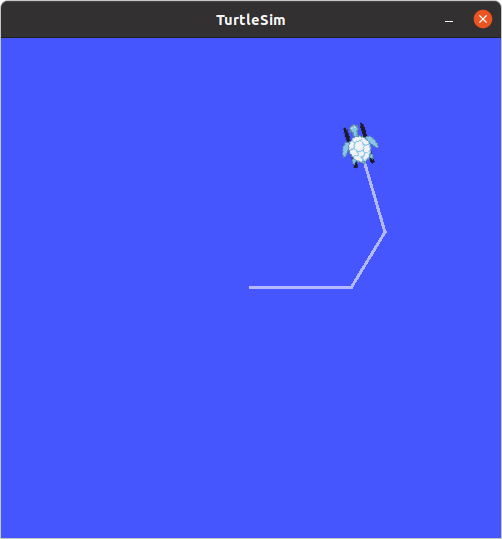
\includegraphics[width=0.3\columnwidth]{turtlesim.png}
 \caption{turtlesimに変身したエルバッキー}
 \end{figure}
 
コマンドは以下の通り。
 \begin{description}
 \item[コンパイル] platex
 \item[pdfへの変換] dvipdfmx
 \end{description}
 
 
 \section{数式のある章}
 
 この章では数式が出てきます。
 
 \begin{equation}
 f = ma     \label{newton}
 \end{equation}
 
 式(\ref{newton})はニュートンの運動方程式です。
 
 \begin{equation}
 E = mc^2   \label{einstein}
 \end{equation}
 
 式(\ref{einstein})はアインシュタインの質量とエネルギーの等価性を示す式です。
 
 \begin{equation}
 H_2 O    \label{water}
 \end{equation}
 
 式(\ref{water})は水の分子式。
 
 \begin{equation}
 x = \frac{-b\pm \sqrt{b^2 - 4ac}}{2a}   \label{second}
 \end{equation}
 
 式(\ref{second})は二次方程式の解の公式です。
 \section{おわりに}
 君は生き残ることができるか? シャアッ!
\end{document}
